\documentclass[10pt,showpacs,showkeys,%preprint,
amsfonts,amsmath,onecolumn,
floatfix,aps,superscriptaddress]{revtex4}
\usepackage{amsfonts,amsmath,array}
\usepackage{graphicx}
\usepackage{bm}
\usepackage{mal}
\usepackage{math}
\usepackage{cancel}

\begin{document}

\title{Multi Spectral Reduction of the Navier-Stokes equations}
\section{Purpose of this document}
This document contains notes for the application of multi-spectral
reduction to the Navier--Stokes equations, which will form the crux
of my thesis.

\section{Introduction}

We begin with the two dimensional Navier--Stokes equations.

What is particularly nice about two-dimensional turbulence is that the
we can represent the velocity by the vorticity, which has only one
non-zero component in two dimensions. The incompressible 2D Navier--Stokes
equations are:
\begin{dmath}
  \theNS, \quad \v\del\cdot\v{u}=0.
\end{dmath}
The vorticity is defined as 
$\v\omega = \del\times\v{u} = (\partial_x u_y - \partial_y u_x )\hat{\v{z}}$
Taking the Fourier transform, we have the following governing equation:
\begin{eqnarray}
  \frac{\partial \omega_{\v k}}{\partial t}
  + \nu_{\v k} \omega_{\v k} 
  &=& \int dp \int dq \frac{\epsilon_{\v{kpq}}}{\v q^2}
  \omega_{\v p}^* \omega_{\v q}^*
  + \v F_{\v k},
  \\
  \epsilon_{\v{kpq}} &=& \(\hat{\v z} \dot \v p \times \v q \)
  \delta\(\v k + \v p + \v q \)
\end{eqnarray}
where $\v F_{\v k}$ represents an external force. The 2D equations conserve
energy and enstrophy, so we would prefere a numerical scheme that maintains
this conservation. That is, the overlap between the two grids should give
identical values for the energy,
\begin{eqnarray}
  \label{E}
  E = \sum_i |u_i|^2,
\end{eqnarray}
and the enstrophy,
\begin{eqnarray}
  \label{Z}
  Z = \sum_i k_i^2|u_i|^2,
\end{eqnarray}
with appropriate weighting factors added for decimated grids.  We will
see that enstrophy conservation, which involes the geometric quantity
$\vk_i$, imposes a restriction on what types of grids we may use and
how we project between them.

% FIXME: out of date paragraph?
One possible arrangement for the grids, wherein the coarse grid is
twice as sparse and rotated by $45^\circ$, is given in figure
\ref{lambdar2}. In the case where a coarse- and fine- grid point share
the same location in Fourier space, equation \eqref{Z} is automtically
satisfied whenever equation \eqref{E} is satisfied. In the arrangement
given in figure \ref{lambdar2}, half of the fine-grid nodes satisfy
the property. For the projection operator to conserve $E$ and $Z$, we
thus need to transfer all of the energy and enstrophy from the
remaining fine-grid nodes to coarse grid nodes.

\section{Decimated Evolution Equation}
We wish to evolve the vorticity field forward in time.  As such, we
need a differential equation that specifies the time-derivative of the
vorticity based upon the vorticity as defined on the desimated grid.
There are two basic choices for this: we either spectrally reduce the
Navier--Stokes equation, or we simply treat the small-scale vorticity
field as periodic in $x$-space and scale the Navier--Stokes equation
by a factor determined by the period we have assumed.

\subsection{Spectrally Reduced Navier--Stokes Equation}
Shell models of turbulence spectrally reduce in a special case, since
the GOY model reduced to the DN model, which is then a fixed point. Id
est, the nonlinear source term is invariant.  Unsurprisingly, the
Navier--Stokes equations present a more difficult problem for spectral
reduction, because the binning of modes removes the perfectly triadic
interaction between wavemodes.

TODO: isn't there something written up about this already?

\subsection{High-Pass Periodic Navier--Stokes Equation}
However, this is not the only map that we may apply to the governing
equation. Taking the spectral vorticity Navier--Stokes equations, each
mode $\v\omega_{\v k}$ has $\v{k} \in \{k_0\(i,j\),i,j=1,\dots ,n \}$, where
$k_0$ is the inverse scale of the $x$-space system, i.e.\ 
$\v{x}\in (0,\pi/k_0)\times(0,\pi/k_0)$ (in our not-really-applied fashion,
we typically take $k_0=1$).  

Let $k_0^{(0)}$ be the spacing of the fine 
grid, and $k_0^{(1)}=\lambda k_0^{(0)}$ be the subgrid spacing, as in 
figure~\ref{lambda2}. The subgrid has 
$\v{k} \in \{2k_0\(i,j\),i,j=1,\dots ,n \}$, which corresponds to 
$\v{x}\in (0,\pi/(2k_0))\times(0,\pi/(2k_0))$. This is equivalent to 
the scaling $\v{x} \rightarrow \v{x}/2$.  If we want to simulate a fluid 
on $\v{x}\in (0,\pi/(k_0))\times(0,\pi/(k_0))$, we simply rescale $\v{x}$ by
a factor of two. This is equivalent to modifying the Navier--Stokes equations
from
\be
\theNS
\ee
to
\be
\ppt{\v{u}} +\v{u}\cdot\lambda\grad\v{u} 
= -\frac{1}{\rho}\lambda\grad P + \nu\lambda^2\nabla^2 \v{u}+ \v{F}.
\ee

The primary advantage of this technique is that it leaves the form of the
governing equation the same.  Thus, all of the computational techniques that 
we have developped for simulating the undecimated Navier--Stokes equations
can still be applied, so long as the grid remains a rectangular lattice in 
Fourier space.

\section{Decimated Grid Geometry}

The undecimated grid geometry is provided to us: it is a rectangular lattice
in Fourier space. The Liouville theorem for the Navier--Stokes equations
implies that decimated grids will only reach the correct equipartition if 
they are decimated uniformly.  Thus, we have a limited number of options in
what type of subgrid we choose to use.  We present two here: a radix-2 scheme
and a radix-4 scheme. % FIXME: and a trivial radix-1 scheme

\subsection{Radix-1 Decimated Grid}
The radix-1 decimated grid is just the original grid; each gridpoint
matches exactly one gridpoint on the undecimated grid (see
Fig.\ ~\ref{lambda1}).  While this is not a practically useful method,
it helps us understand the effect that the multispectral method has on
the accuracy of the simulation.

For this method to be non-trivial, we must have a different fewer
modes on the large-scale grid than on the small-scale grid. The
projection and prolongation operators are simply copying the data from
one gridpoint to the corresponding gridpoint at the same location in
Fourier space.  The nonlinearity is only slightly complicated by the
fact that we must remove low-low-low interactions from the
high-wavenumber grid. This is done by calculating the nonlinear
interaction of all modes on the high grid, which we denote
$\text{NL}_{\text{high}}$, which can be done with a fast convolution
over all modes.  Then calculatethe nonlinearity on the subset of modes
from the high-wavenumber grid that are in the low-wavenumber grid,
denoted $\text{NL}_{<,\text{high}}$ by doing a fast convolution over
the subset of modes which match modes on the low grid.  The nonlinear
source term for the high grid is then
$\text{NL}_{>,\text{high}} = \text{NL}_{\text{high}} - \text{NL}_{<,\text{high}}$.


Consider the integration method given in (REF: MSc) single-step
numerical integrators such as a Runge-Kutta method of order $n$.
Using a radix-1 decimated high grid, and an undecimated low grid, we
would evolve the low grid forward in time, project onto the high grid,
move this forward in time, and then prolong onto the low grid.  The
goal is to have the decimated system behave like a full-resolution
undecimated system.  In this case, the full-resolution undecimated
system is just the high-wavenumber grid!  Were we to ignore the low
grid and not high-pass filter the high-grid nonlinearity, we would
have the original system, with the important disctinction that all
source terms would be calculated at each stage of the Runge-Kutta
integrator.  With two grids, the high grid is affected by low-low-low
interactions only at the end of the time step; as such, we expect that,
while the sub-integrators have error $\O\(\tau^{n+1}\),$ the low-low-low
interactions are only $\O\(\tau^1\)$.

\begin{figure}[htbp]
  \begin{center}
    \includegraphics[width=0.5\textwidth]{figures/lambda1}
    \caption{Radix-1 Decimated Grid.}
    \label{lambda1}
  \end{center}
\end{figure}


\subsection{Radix-2 Decimated Grid}
The radix-2 decimated grid has half the number of modes per unit area
in Fourier space as does the undecimated grid.  In order to decimate uniformly,
we remove every mode with two odd indices, as shown in Fig.\ ~\ref{lambdar2rot}.
If the undecimated grid is a square lattice, then the decimated grid is also
a square lattice, as can be seen in Fig.\ \ref{lambdar2}; it has been
stretched by a factor of $\sqrt{2}$ and rotated by $45\ensuremath{^\circ}$.
Given the same number of modes on the undecimated grid and the decimated
subgrid, a radix-2 decimation scheme extends the maximum wavenumber to 
$\sqrt{2}$ times that of the undecimated grid alone. As such, it seems wise
to use a larger number of modes in the subgrid than in the undecimated grid.


\begin{figure}[htbp]
  \begin{center}
    \includegraphics[width=0.5\textwidth]{figures/lambdar2rot}
    \caption{Radix-2 Decimated Grid.}
    \label{lambdar2rot}
  \end{center}
\end{figure}
\begin{figure}[htbp]
  \begin{center}
    \includegraphics[width=0.5\textwidth]{figures/lambdar2}
    \caption{Rotated Radix-2 Decimated Grid.}
    \label{lambdar2}
  \end{center}
\end{figure}

\subsubsection{Projection}
Nodes on the fully-resolved grid may either
\begin{enumerate}
\item \label{rad2co}
  be co-incident in Fourier space witha a mode on the decimated grid, or
\item \label{rad2four}
  be equidistant from four modes on the decimated grid.
\end{enumerate}
The co-incident grid points are simple to project: since the source
and destination modes have the same wavenumber, any transfer of
energy-conserving projection will automatically conserve enstrophy as
well.

For case~\ref{rad2four}, enstrophy conservation is more difficult.
Let mode $K$ have energy $E$ and enstrophy $K^2E$.  Suppose that we
require modes on opposite sides of the mode on the fully-resolved grid
conserver energy and enstrophy pair-wise, as in figure~\ref{rad2cross}. 
\begin{figure}[htb]
  \begin{center}
    \includegraphics[width=0.5\textwidth]{figures/rad2cross}
    \caption{Projection diagram.}
    \label{rad2cross}
  \end{center}
\end{figure}
Enstrophy conservation is guaranteed if 
% FIXME: check this for correct indices
\begin{dmath}
  \alpha = \frac{k^2 -k_3^2}{ k_1^2 -k_3^2},
  \quad
  \beta = \frac{k^2 -k_2^2}{ k_0^2 -k_2^2}.
\end{dmath}
This is possible if $k_1^2 \neq k_3^2$ and $k_0^2 \neq k_2^2$, which
happens if mode $k$ is not on the $k_x$ or $k_y$ axis. %FIXME: what to do?




\subsubsection{Prolongation}
Once we have evolved the system on the coarse grid, we need to
repopulate the modes that were evacuated by projection.  Since every
coarse-grid mode has a corresponding fine-grid mode with the same
wavevector, the requirements of energy and enstrophy conservation
allow for a variety of repopulation schemes.  Two obvious choices come
immediately to mind:
\begin{enumerate}
\item
populate fine-gride modes with no corresponding coarse mode, using the inverse
of the projection operator to ensure conservation of invariants, 
\item
transfer all the energy from the coarse modes to the corresponding fine 
mode, setting all other modes to zero.
\end{enumerate}
An obvious choice is the combination of these two possibilities, using 
the ratio of fine-grid energies to determine how much energy is transferred
to what modes. The prolongation operator diagram is shown in figure 
\ref{prolside}, which gives the names of the modes that we will be using
in this subsection.
\begin{figure}[htb]
  \begin{center}
    \includegraphics{figures/prolside}
    \caption{Side-view of projection.}
    \label{prolside}
  \end{center}
\end{figure}

\subsubsection{Prolongation choice 1}
An ideal solution would be to redistribute energies from the coarse grid
to the fine grid so that the original ratio of energies in the modes
of the fine grids is unaffected by the evolution of the coarse grid.
That is, a coarse mode $U_+$ was populated with energy with ratio 
$E_0:E_+:E_{++}$, with energy from the fine-grid modes $u_0$, $u_+$, 
and $u_{++}$, respectively, i.e.\ , before projection, we had
\begin{eqnarray}
  E_0:E_+:E_{++} = u_0^2: u_+^2: u_{++}^2
\end{eqnarray}
and we would like to ensure that this is the case after prolongation. 

However, energy and enstrophy conservation relies on energies being 
distributed in ratios $\alpha$ and $(1-\alpha)$, which may be impossible if,
for example, if only one of $U_-$ and $U_+$ drops to zero.

\subsubsection{Prolongation choice 2}
During projection, the energy of mode $U_-$ is determined by the 
geometric factors $\alpha_i$ and the energies of the fine-grid modes.
That is,
\begin{eqnarray}
  U_-^2 &=& \(1-\alpha_{--}\)E_{--} + E_- + \alpha_0E_0
  \\
  U_+^2 &=& \(1-\alpha_0\)E_0 + E_+ + \alpha_{++}E_{++}.
\end{eqnarray}
Let $\hat U_i$ denote $U_i$ after the completion of a Runge--Kutta time step.
From this, we can determine the energy that the fine modes should have.
We choose to remove energy from $U_-$ and $U_+$ so that
\begin{eqnarray}
  u_0^2= E_0 \leftarrow u_0^2 \times
  \min\{\frac{\hat U_-^2}{U_-^2},\frac{\hat U_+^2}{U_+^2}\}.
\end{eqnarray}
This guarantees that we do not attempt to remove more energy from
coarse modes than is present. Any remaining energy is then deposited
into the fine-grid modes that coincide with coarse-grid modes in
Fourier space, which automatically conserves both $E$ and $Z$.

\subsection{Radix-4 Decimated Grid}

\begin{figure}[htb]
  \begin{center}
    \includegraphics[width=0.5\textwidth]{figures/lambda2}
    \caption{Radix-4 Decimated Grid.}
    \label{lambda2}
  \end{center}
\end{figure}

% FIXME: out-of-place
However, scaling the grids by a factor introduces a restriction on the
geometry that we can use. In particular, the imposition of a square
lattice will lead to a problem with projection/prolongation near the
spectral origin: fine-grid modes adjacent to the origin can only
project their energy onto coarse modes with higher wavenumber, which
breaks enstrophy conservation. This may be rectified by reintroducing
the spectral origin, which is not evolved by the spectral
Navier--Stokes equations, as a buffer into which some energy may be
depositied.  In this case, every fine-grid mode is has at least one
adjacent coarse-grid mode with higher $k$ and one adjacent coarse-grid
mode with lower $k$.

\subsubsection{Projection and Prolongation}
Nodes on the fully-resolved grid may either
\begin{enumerate}
\item \label{ontop}
  be co-incident in Fourier space with a mode on the decimated grid,
\item \label{rowcol}
  lie on the same row or column between two modes on the decimated grid,
\item \label{4cross}
  or be equidistant from four modes on the decimated grid.
\end{enumerate}

Projecting is easy in case \ref{ontop}; since the resolved and
decimated wave-vectors are the same, copying the energy from one grid
to the next preserves energy and enstrophy automatically.

In case \ref{rowcol} (figure \ref{rad4row}) energy sent to smaller-$k$
must be compensated by energy sent to larger-$k$ in order to conserve
vorticity.  Let $E$ be the energy and $K^2E$ the enstrophy in the mode
on the fully resolved grid.
\begin{figure}[htb]
  \begin{center}
    \includegraphics{figures/rad4row}
    \caption{Radix-4 row/colum projection.}
    \label{rad4row}
  \end{center}
\end{figure}
If a fraction $\alpha$ of the energy is
sent to the mode at $k_1$, then energy conservation requires that
$1-\alpha$ of the energy be sent to the mode at $k_2$.  The enstrophy
after projection is $k_1^2\alpha E+ k_2^2 (1-\alpha)E$.  Solving for 
$\alpha$, we get
\begin{dmath*}[compact]
  \alpha=\frac{K^2-k_2^2}{k_1^2-k_2^2}.
\end{dmath*}
If $k_1^2=k_2^2\neq K^2$, it isn't possible to conserve enstrophy under
projection.  Fortunately, this is impossible with radix-4 decimation.
%FIXME: prove this.

Case~\ref{4cross} has four projection coefficients.  The constraints
of energy and enstrophy conservation leave this system undetermined.
If we arbitrarily decide that projection in opposite directions must
pair-wise conserve energy and enstrophy, we are left a projection
diagram as in figure \ref{rad4cross}.
\begin{figure}[htb]
  \begin{center}
    \includegraphics{figures/rad4cross}
    \caption{Radix-4 equidistant projection.}
    \label{rad4cross}
  \end{center}
\end{figure}
Following case~\ref{rowcol}, we solve for $\alpha$ and $\beta$ using
energy and enstrophy conservation:
\begin{dmath*}[compact]
  \alpha=\frac{K^2-k_3^2}{k_1^2-k_3^2}, 
  \qquad 
  \beta=\frac{K^2-k_4^2}{k_2^2-k_4^2}.
\end{dmath*}
In this case, however, the denominator vanishes for either $\alpha$ or $\beta$
is the mode $K$ lies on a line which goes through the origin at 45$^\circ$.


Due to this problem (which also occurs on radix-2 projection), %FIXME:
ref we propose an alternative solution.  Let
$L=\{k_i,i=1,2,3,4|k_i^2<K^2 \}$ and $H=\{k_i,i=1,2,3,4|k_i^2>K^2 \}$.
We are guaranteed that $H$ and $L$ have at least one element, and that
$\abs{H} + \abs{L}=4$.  Suppose that we put energy $E_L$ into the
modes in $L$ and $E_H$ into the modes in $H$, which, is then divided 
among the modes to in a stat-mech equipartition. Thus, for modes
in set $S=L$ of $S=H$, we have $\a=\a_S$, $\b=\b_S$.

Suppose that we send $\abs{H}S$ of energy to the modes in $S$,\dots

Nah, forget that: Let's just equipartition the thing. We start out
with energy $E$ and enstrophy $K^2E$. In equiparition, mode $k_i$ has
enstrophy $1/\(\alpha/k_i^2 + \beta\)$. Thus, the total energy and
enstrophy are
\begin{dmath*}[compact]
  E = \sum_{i} \frac{1}{\alpha + \beta k_i^2},
  \quad
  Z = \sum_{i} \frac{k_i^2}{\alpha + \beta k_i^2}
\end{dmath*}
This gives us two equations with two unknowns, which
we should be able to solve.  Amusingly, this is actually an exercise 
from math 655, and we can eliminate $\a$: 
\begin{dmath*}
  \a=\frac{\abs{S}/2 - \beta Z}{E}.
\end{dmath*}
The energy equation is (with $\abs{S}=n$ and assuming $E\neq 0$) then 
\begin{dmath*}
  1 = \sum_{i} \frac{1}{n/2+ \b\( E k_i^2- Z\) }.
\end{dmath*}
Multiply both sides by $\prod_i \[n/2+ \b\( E k_i^2- Z\)\]$ yields
\begin{dmath*}
  \prod_i \[n/2+ \b\( E k_i^2- Z\)\]
  = \sum_{i} \prod_{j\neq i} \[n/2+ \b\( E k_j^2- Z\)\].
\end{dmath*}
In the case that $n=2$, we can solve this explicitly:
\begin{dmath*}[compact]
  \prod_{i=1,2} \[1+ \b\( E k_i^2- Z\)\]
  = \sum_{i=1,2}  \[1+ \b\( E k_i^2- Z\)\] 
  \implies \b^2 = \prod_{i=1,2} \frac{1}{E k_i^2 -Z}
\end{dmath*}


\subsubsection{Boundary modes}
The boundary modes should be accounted for during synchronization: they
are part of the overlapping set of modes, albeit only fractionally.

The radix-2 and radix-4 cases present two boundary, coarse-grid modes
that are not fully redundant with fine-grid modes.  In the radix-4
case, we have one side of a row- or column-projection, as shown in
figure~\ref{bpair}. In this case, the coarse-grid mode should
represent half of the fine-grid mode. A problem arises in
projection/prolongation, in that projecting onto the coarse grid
should replace the state of the coarse modes with a state derived from
the fine grid.  Since the coarse-grid mode isn't entirely determined
by the fine grid, we can only ``half-replace'' the mode. A symmectric
synchronization, i.e.\ rescaling, can get around this by just sending
the appropriate fraction of the energy to the coarse-grid mode.  The
problem remains of how to ensure that the grids are synchronized at
the beginning of the time-step, but this should (?) be possible to do.


\begin{figure}[htbp]
  \begin{center}
    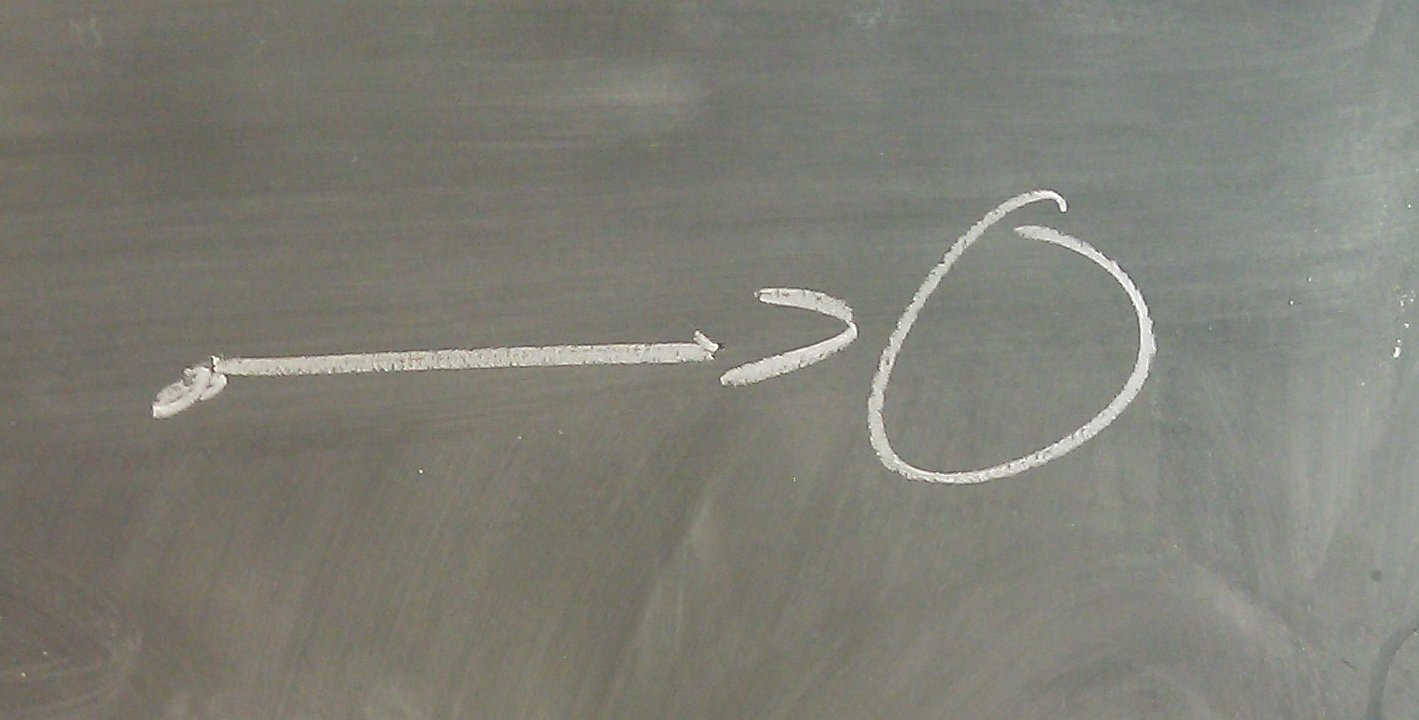
\includegraphics[width=0.4\textwidth]{figures/bpair.jpg}
    \caption{half of a 2-to-1 interaction}
    \label{bpair}
  \end{center}
\end{figure}
\begin{figure}[htbp]
  \begin{center}
    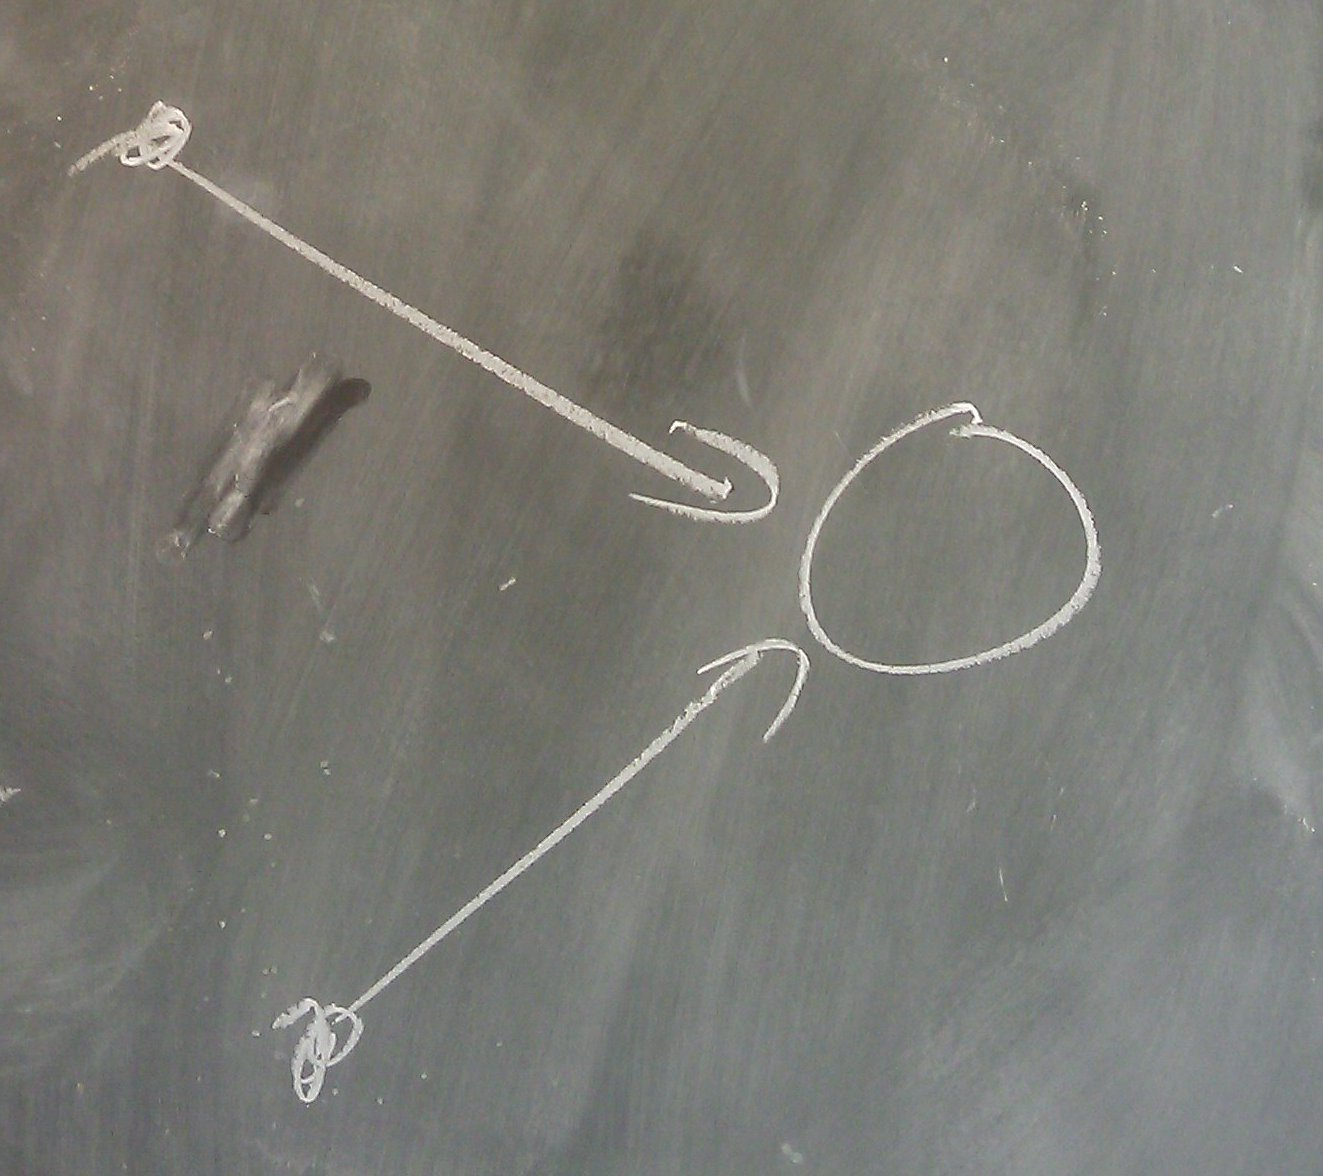
\includegraphics[width=0.4\textwidth]{figures/bquad.jpg}
    \caption{half of a 4-to-1 interaction}
    \label{bquad}
  \end{center}
\end{figure}

%Also, see note 2010-06-24

\subsection{Calculating the Nonlinear Source Term on Decimated Grids}

\subsubsection{Using Spectral Reduction}

TODO: How would you use spectral reduction here?  Just bin things?
Does one end up with a convolution, or just some nasty $\O(n^2)$ sum?

\subsubsection{Using High-Pass Periodicity}

Since the grids are just scaled square lattices, the nonlinearity may
be calculated by simply changing the parameters in the spectral
(spectrally bounded, discrete) Navier--Stokes equations.  However,
there is one important difference: we must avoid double-counting
interactions which appear in both the fully-resolved and
high-wavenumber grids.  Preferring to keep as many interactions from
the fully-resolved grid as possible, this amounts to removing
low-low-low interactions from the decimated grid.  Fortunately, (I
think) the low-low-low interactions are just the scaled interactions
for a subset of the decimated grid.  Thus, they are a convolution if
the normal nonlinearity is a convolution, and are amenable to
calculation using so-called fast convolutions.  w00t.

\section{Grid Synchronization}

There are two methods: rescaling and  projection/prolongation.

\subsection{Rescaling}
I talked about this in my MSc thesis, but was told not to do it then.  Now 
people seem to like it.
\begin{figure}[htbp]
  \begin{center}
    \includegraphics{figures/symstep4}
    \caption{Time-stepping with rescaling}
    \label{symstep4}
  \end{center}
\end{figure}
Let $S_1$ be a set of modes, with $S_1\subset\Omega_1$, which corresponds
to the set of modes $S_2\subset\Omega_2$. Let $E_i$ be the energy of the
modes in $S_i$, $i=1,2$. At the beginning of the time step, $E_i(t)$ are
all equal, wlog. Let $\D E_i$ denote the change in energy of the set
$S_i$ from time $t$ to $t+\t$. We must scale the energies of the modes
so that the change from each grid is accounted for. That is, for
each mode $\w$, we need
\begin{eqnarray}
  \sum_{\w\in S_i}\half\abs{\widetilde\w(t+\t)}^2 = E_i 
\end{eqnarray}
to be scaled up so that
\begin{eqnarray}
  \sum_{\w\in S_i}\half\abs{\w(t+\t)}^2 
  = E(t) + \sum_j \D E_j
  = E_i(t+\t) + \sum_{j\neq i} \D E_j.
\end{eqnarray}
That is, each mode in $S_i$ must be scaled as:
\begin{eqnarray}
  \w(t+\t)&=&\widetilde\w(t+\t)
  \sqrt{\frac{E_i(t) + \sum_{j} \D E_j}{E_i(t+\t)}}
  \\
  &=&\widetilde\w(t+\t) \sqrt{
    \frac{\half\abs{\w(t)}^2 
      + \sum_j\(\half\abs{\widetilde\w_j(t+\t)}^2  -  \half\abs{\w(t)}^2\)}
         {\half\abs{\widetilde\w(t+\t)}^2}
  }
  \\
  &=&\widetilde\w(t+\t) \sqrt{
    \frac{\abs{\w(t)}^2 
      + \sum_j\(\abs{\widetilde\w_j(t+\t)}^2  -  \abs{\w(t)}^2\)}
         {\abs{\widetilde\w(t+\t)}^2}
  }
  \\
  &=&\frac{\widetilde\w(t+\t)}{\abs{\widetilde\w(t+\t)}}
 \sqrt{
   \abs{\w(t)}^2 + \sum_j\(\abs{\widetilde\w_j(t+\t)}^2  -  \abs{\w(t)}^2\)
  }
\end{eqnarray}
It is important that $E_i(t) + \sum_{j} \D E_j\geq 0$, because otherwise
we would encounter a negative root, and the energy would become complex
(to say nothing of branch-cut issues).  Since the energy change can
be approximated as a polynomial in the time-step $\t$, we will be able
to reduce the time-step so that the resulting energy is non-negative. This
only takes a finite number of time-step reductions, because we eventually
hit machine-precision, whereat a decrese in $\t$ so reduces the energy
change as to be zero. FIXME: we can prove this.

Synchronization via rescaling can be extended to more than two grids in
a straightforward fashion: the sums above were left in a general format,
so just add more grids. This may add restrictions on the timestep, since
we can now have more than one grid removing energy from a corresponding 
set of modes. It is worthwhile noting that this case was never observed 
for shell models of turbulence, and happen only with probability 0 (or
whatever the discrete analogue of zero probability is, probably something
like machine precision or something like that).

But what do we do with the phase? FIXME

\subsection{Projection/Prolongation}
\begin{figure}[htbp]
  \begin{center}
    \includegraphics{figures/timestep8}
    \caption{Time-stepping with projection/prolongation}
    \label{timestep8}
  \end{center}
\end{figure}
\subsubsection{Mode-centric synchronization}
Let $A$ be a set of modes on grid $a$ which correspond to the modes in
set $B$ on grid $b$.  We wish to project/prolong between grids $a$ and
$b$.  Projection and prolongation are assymetric operations.  Let
$||.||$ denote an (energy? enstrophy?) norm which maps a set of modes
to the positive real axis. Assume that $||A(t)||=||B(t)||$ at time
$t$. We advance, say, modes in $a$ to time $t+\t$. Since the modes in
$A$ represent the same physical quantities as those in $B$, we need to
impose the change from $A(t) \rightarrow \widetilde{A}(t+\t)$ onto $B$. If
our norm is the energy of the modes, we can just set
\begin{dmath}
  \widetilde{B}(t) = B(t) \times \frac{||\widetilde{A}(t+\t)||}{||A(t)||}.
\end{dmath}
Then we advance $\widetilde{B}(t)$ to time $t+\t$:
$\widetilde{B}(t)\rightarrow B(t+\t)$.  This change must now be imposed on $A$:
\begin{dmath}
  A(t+\t) = \widetilde{A}(t+\t)\times \frac{||B(t+\t)||}{||\widetilde{B}(t)||}.
\end{dmath}

\subsubsection{Transform-centric rescaling}
The spectral Navier--Stokes equations are derived by projecting the
solution onto a basis which consists of Fourier modes.  The decimated
equation is just the projection onto a different decimated
basis. Therefore, synchronizing the grids should be done using the
same projection operator, the Fourier transform.

The decimated modes have wavenumbers 
$\{e^{i k \cdot x}, k \in 2\mathbb{Z}\times2\mathbb{Z}\}$.
Interpolation via Fourier transform is done as follows:
\begin{dmath}
  \text{fine grid} \xrightarrow{\text{fft}^{-1}} x\text{-space}.
  \xrightarrow{\text{fft}} \text{decimated grid}
\end{dmath}
The fine grid to $x$-space transform is a bijection, but the transform
to the decimated grid is not one-to-one, since we restricted to modes
with even indices. The effect is to simply identify the coincident
modes between grids, and copy the information between them.  The
Fourier transform, used in justifying the scheme, can be avoided at
the implimentation level.

Let $\Omega_{\text{f}}$ denote wavenumbers on the fine frid, and
$\Omega_{\text{c}}$ the wavenumbers on the coarse grid. Then we can
consider the system to be $\Omega_{\text{f}} \cup \Omega_{\text{c}}$.
The linear source and external forces are simple to account for.
The nonlinear interaction is more complicated.  There are a number
of cases.
\begin{enumerate}
  \item 
    $\Omega_{\text{f}} \times \Omega_{\text{f}}\rightarrow \Omega_{\text{f}}$\\
    These interactions are included in the fine-grid nonlinear calculation.
  \item 
    $\Omega_{\text{c}} \times \Omega_{\text{c}}\rightarrow \Omega_{\text{c}}$\\
    These interactions are included in the coarse-grid nonlinear calculation.
  \item 
    $\Omega_{\text{c}} \times \Omega_{\text{c}}\rightarrow \Omega_{\text{f}}$\\
    Since the coarse grid contains only even modes, these modes only beat
    to influence even modes on the fine grid.  These modes are also part
    of the coarse grid.  Therefore, these interactions are part of
    $\Omega_{\text{c}} \times \Omega_{\text{c}}\rightarrow \Omega_{\text{c}}$.
  \item
    $\Omega_{\text{f}} \times \Omega_{\text{f}}\rightarrow \Omega_{\text{c}}$\\
    This is a more complicated case. The even-even-to-even interaction
    is included in the coarse-coarse interaction, and the even-odd-to-odd
    interaction influences odd modes which are not part of the coarse grid.
    But the odd$\times$odd$\rightarrow$even interaction still needs to
    be taken into account, or we will decrease the coupling between the
    two grids.
    
    Since the dimensions of the grids are odd, there is no bijection
    between these interactions and those in 
    $\Omega_{\text{c}}\cap \Omega_{\text{f}} \times 
    \Omega_{\text{c}}\cap \Omega_{\text{f}}$, which would result in the 
    interactions on the axes being double-counted. We might be able to
    simply not high-pass filter the coarse nonlinear interaction, and 
    elminate the double-counting by removing the interaction on the 
    axes, which would just take two one-dimensional convolutions. 
    (FIXME: check this.) This would be a simple enough calculation
    as to be feasible without using a fast-convolution algorithm, which
    might be unavailable for this geometry. (FIXME: check this)
    
  \item
    $\Omega_{\text{f}} \times \Omega_{\text{c}}\rightarrow \Omega_{\text{c}}$\\
    This odd terms are not part of the system, and the even terms are
    part of the coarse-coarse interaction.
  \item
    $\Omega_{\text{f}} \times \Omega_{\text{c}}\rightarrow \Omega_{\text{f}}$\\
    What about this?
\end{enumerate}

Transform-centric synchronization offers some interesting possibilities.
Since we deal only with coincident modes, we can just copy the value 
of the mode from one grid to another without having to make any
approsimations.  This eliminates many ambiguities as compared with the
``area''-based synchronization scheme. Also of note is that, after
calculating the source term, and assuming that we maintain all nonlinear
interaction for $\Omega_{\text{f}} \cup \Omega_{\text{c}}$, then the 
combined system does not modify the ergodicity of the original system:
we simply project the $x$-space system onto 
$\Omega_{\text{f}} \cup \Omega_{\text{c}}$, which maintains ergodicity
assuming that all modes are (well-enough?) connnected by the nonlinearity.
So, we should be able to add source terms without ruining equipartition!
FIXME: check.

The basic idea here is that, if we express the velocity field as a linear
combination of modes in 
\begin{eqnarray}
  S\doteq\cup_i \Omega_i
\end{eqnarray}
but we only have the individual grids $\Omega_i$. The nonlinear interactions
in $S$ are from the set
\begin{eqnarray}
  S\times S = \(\cup_i \Omega_i\)\times \(\cup_j \Omega_j\),
\end{eqnarray}
but we only have access to 
\begin{eqnarray}
  \cup_i\(\Omega_i \times \Omega_i\) 
  \subsetneq 
  \(\cup_i \Omega_i\)\times \(\cup_j \Omega_j\).
\end{eqnarray}
Options for dealing with this:
\begin{enumerate}
  \item ignore the missing interactions
  \item strengthen some of the interactions to compensate for the
    missing interactions, or
  \item calculate the missing interactions.
\end{enumerate}

Ignoring things is often a perfectly reasonable way to deal with one's
problems, at least as a first attempt, and this first option is
somewhat enticing due to its ease of implementation.  However, some
of the graphs of the spectra seem to show a bottleneck at the
intergrid boundary, so this might not be something that we can simply
overlook.  Later, more-resolved and statistically stationary simulations
will shed more light on whether this is an actual problem.

The second option might be ok; for the overlap, the missing odd modes
can be replaced by the even modes (there isn't a bijection, but we're
only off by a lower-dimensional array, which might still be accounted 
for) and these triads can be strengthened. This shouldn't be an overly 
difficult computation; at least it can be done as a convolution, and 
perhaps even without having to do a separate convolution.

The third option is quite appealling. At least for the low$\times$low
interaction, since this can be done by a conventional padded fast
convolution, keeping the aliases, which are just the missing terms. 
The high$\times$high interactions can be done via a fast convolution
only if we use a grid that keeps the missing low-wavenumber interactions
and extends to reach high wavenumbers.  This misses the point of 
the multispectral method entirely, as we end up just having a full grid.
This might be something that we need to do either as a modified
convolution, or simply by hand (i.e.\ not using a fast convolution method).
The high$\times$low interactions face a similar problem. 

All of this stuff needs looking into; the triad interaction puts an
interesting restraing on the geometry.

\end{document}
